\documentclass[10pt,twocolumn]{article}
\usepackage[top=0.5in,bottom=0.5in,left=0.55in,right=0.55in]{geometry}
\usepackage{graphicx}
\usepackage{amsmath}
\usepackage{amssymb}
\usepackage{hyperref}
\usepackage{booktabs}
\usepackage{microtype}

\graphicspath{{../results/}}

\title{\vspace{-3.2em}\textbf{\large SafeExit-RL: Adaptive Fire Evacuation Guidance under Partial Observability and Dynamic Congestion}\vspace{-0.9em}}
\author{
  \textbf{Lokesh Motwani} \quad \textbf{Jenish Thakkar} \\
  \small Department of Computer Science and Engineering \quad Repository: \url{https://github.com/lokesh-2406/SafeExit-RL}
}
\date{}

\begin{document}
\maketitle

\begin{abstract}
Centralized, omniscient routing in building fire evacuation fails under realistic sensor degradation and crowd stampedes. We present \textbf{SafeExit-RL}, an adaptive evacuation framework formulated as a POMDP. We benchmark a Deep Q-Network (DQN) with a 14-dimensional continuous layout-invariant state and Relative Tabular Q-learning against Static Shortest Path (BFS) and Reactive Replanning (Dijkstra) across three regimes: (1) immediate egress, (2) 20-step pre-evacuation delay with stationary hazard exposure, and (3) zero-shot cross-layout transfer to an unseen multi-wing building. Under severe sensor noise ($\sigma{=}0.3$), DQN maintains 97.9\% evacuation success and 2.59 cumulative hazard exposure, whereas Static Shortest Path degrades to 87.5\% success with 3.74 exposure. Under a 20-step pre-evacuation delay, DQN achieves 100\% success and 0.06 post-delay exposure, outperforming Reactive Replanning (95.0\% success, 9.69 exposure). Finally, zero-shot transfer highlights the structural distinction between local perception-action RL and global topological search.
\end{abstract}

\section{Introduction}
Indoor fire evacuation requires fast, risk-averse routing under expanding flame fronts, toxic smoke, and moving evacuee crowds. Classical guidance relies on static exit signage or global shortest-path algorithms~\cite{safestep}. However, static paths can steer occupants into compromised halls, and central planners fail when communication links fail or fire blocks predicted routes~\cite{pomdp_planning}.

While Reinforcement Learning (RL) enables dynamic route adaptation~\cite{rl_evacuation}, prior work frequently presumes ideal sensing: full-grid hazard awareness without delay or noise. In real buildings, sensors have finite coverage ($\rho{=}2$), Gaussian noise ($\sigma$), and telemetry latency ($\tau$). Moreover, occupant panic and herding generate dynamic choke points. \textbf{SafeExit-RL} addresses this via: (1) realistic sensing with noise, staleness, and radius limits; (2) crowd-coupled congestion; (3) rigorous pre-evacuation delay exposure accounting; and (4) coordinate-invariant representations for zero-shot transfer.

\section{POMDP Problem Formulation}
We formulate fire evacuation as a POMDP $\langle \mathcal{S}, \mathcal{A}, \mathcal{T}, \mathcal{R}, \Omega, \mathcal{O}, \gamma \rangle$. The environment state $s_t = (p_t, H_t, C_t, t) \in \mathcal{S}$ tracks occupant position $p_t \in \mathcal{G}$, true hazard field $H_t: \mathcal{G} \to [0, 1]$, crowd positions $C_t: \mathcal{G} \to \mathbb{N}$, and simulation tick $t$. Within sensing radius $\rho{=}2$, the agent receives observation $o_t \in \Omega$:
\begin{equation}
o_t = \left( p_t,\; \{\hat{h}_t(u)\}_{u \in \mathcal{N}_\rho},\; \{c_t(u)\}_{u \in \mathcal{N}_\rho},\; s_t,\; b_t,\; w_t \right)
\end{equation}
where $\mathcal{N}_\rho(p_t) = \{u \in \mathcal{G} \mid \|u - p_t\|_\infty \le \rho\}$. Observed hazard is corrupted by Gaussian noise: $\hat{h}_t(u) = \mathrm{clip}(H_t(u) + \epsilon,\, 0,\, 1)$ with $\epsilon \sim \mathcal{N}(0, \sigma^2)$, refreshed every $\tau$ steps. Unobserved cells retain stale internal belief $B_t(u)$ with staleness $s_t(u) = t - t_{\mathrm{last}}(u)$. Exit bearing $b_t = (b_{dr}, b_{dc}) \in [-1, 1]^2$ is a unit vector pointing toward the nearest believed-safe exit. The action space $\mathcal{A} = \{\text{left}, \text{right}, \text{forward}, \text{backward}, \text{wait}\}$ comprises 5 discrete actions with deltas $(0, -1)$, $(0, 1)$, $(-1, 0)$, $(1, 0)$, and $(0, 0)$.

\subsection{State Representations}
\textbf{1) DQN (14D Continuous):} Feature vector $\phi(o_t) \in \mathbb{R}^{14}$ invariant to absolute spatial coordinates:
\begin{equation}
\phi(o_t) = \left[ w_t,\; b_t,\; \bar{h}_t,\; \hat{h}(p_t),\; \hat{h}_{\mathrm{adj}},\; C_{\mathrm{total}}/10,\; c(p_t)/5 \right]
\end{equation}
where $w_t \in \{0, 1\}^4$ is 4-directional local wall traversability (forward, backward, left, right); $b_t \in [-1, 1]^2$ is exit bearing; $\bar{h}_t$ is mean believed hazard in $\mathcal{N}_\rho$; $\hat{h}(p_t)$ is believed hazard at $p_t$; $\hat{h}_{\mathrm{adj}} \in [0, 1]^4$ are cardinal neighbor hazards; $C_{\mathrm{total}} = \sum_{u \in \mathcal{N}_\rho} c_t(u)$; and $c(p_t)$ is local crowd density at $p_t$.

\textbf{2) Relative Tabular Q-learning:} Discrete tuple $s_t^{\mathrm{tab}} = (w_t, \mathrm{bin}(\bar{h}_t), \mathrm{bin}(C_{\mathrm{total}}), \mathrm{dir}(b_t))$ with 16 wall states ($w_t$), 4 hazard tiers ($[0, 0.05), [0.05, 0.2), [0.2, 0.5), [0.5, 1]$), 4 crowd tiers ($0, 1, 2, \ge 3$), and 5 bearing directions ($\mathrm{dir}(b_t)$), totaling 1,280 states. Unseen states during evaluation default to $\mathrm{dir}(b_t)$.

\subsection{Reward Engineering}
The scalar reward balances progress, hazard avoidance, congestion avoidance, and terminal exit arrival:
\begin{equation}
r_t = R_{\mathrm{prog}} + R_{\mathrm{haz}} + R_{\mathrm{cong}} + R_{\mathrm{term}}
\end{equation}
where $R_{\mathrm{prog}} = -1.0 \cdot \mathbb{I}_{\mathrm{wall}} - 0.3 \cdot \mathbb{I}_{\mathrm{revisit}} - 0.1 \cdot \mathbb{I}_{\mathrm{step}}$ penalizes wall collisions ($-1.0$), revisiting cells ($-0.3$), and elapsed time ($-0.1$); $R_{\mathrm{haz}} = -B_t(p_t) \in [-1, 0]$ penalizes perceived hazard at the current cell using internal belief $B_t$; $R_{\mathrm{cong}} = -0.2 \cdot c_t(p_t)$ penalizes occupancy in cells crowded by NPCs; and terminal exit reward is:
\begin{equation}
R_{\mathrm{term}} = 20.0 \cdot \max(0,\, 1 - E_{\mathrm{post}}) \cdot \mathbb{I}(p_t \in \mathcal{E})
\end{equation}
scaled strictly by post-delay ground-truth cumulative exposure $E_{\mathrm{post}} = \sum_{k=1}^{T_{\mathrm{post}}} H_k(p_k)$. Crucially, pre-evacuation exposure $E_{\mathrm{pre}}$ accumulated while stationary during delay does not attenuate $R_{\mathrm{term}}$, preserving learning gradients for active egress routing.

\section{Environment Dynamics and Baselines}
The building is an $H \times W$ grid of walls ($\#$), corridors ($\cdot$), fire origin ($F$), and exits ($E$). Fire spreads via an analytical radial sigmoid proxy: $r(t) = 20.0 / (1 + e^{-0.05(t - 60)})$, with ground-truth cell hazard $H_t(u) = \max(0,\, 1 - \|u - u_0\|_2 / r(t))$. $N = 10$ NPCs execute biased random walks toward nearest exits. If local hazard $>0.2$, NPCs panic with probability $p_{\mathrm{panic}}$, picking random directions; with probability $p_{\mathrm{herd}}$, NPCs herd toward nearby peers, inducing dynamic blockages. Episodes end on exit arrival ($p_t \in \mathcal{E}$) or at $T_{\mathrm{max}} = 200$ active steps.

\textbf{Primary Comparison Methods:}
(1) \textbf{DQN:} 2-layer MLP (hidden 64, ReLU), replay buffer $10^4$, batch 64, $\gamma = 0.95$, target sync every 100 steps, Adam ($\mathrm{lr} = 10^{-3}$), $\epsilon$-decay $1.0 \to 0.05$ over 1,500 episodes, Huber loss.
(2) \textbf{Relative Tabular Q:} Q-table over 1,280 states, $\alpha = 0.1$, $\gamma = 0.95$, $\epsilon$-decay over 1,500 episodes.
(3) \textbf{Static Shortest Path (Static SP):} Offline BFS at $t=0$; executes blindly without replanning.
(4) \textbf{Reactive Replanning:} Online Dijkstra replanning every $k=5$ steps with edge costs $w(u, v) = 1.0 + 10.0 \cdot B_t(v) + 2.0 \cdot c_t(v)$.

\section{Experimental Evaluation and Results}

\begin{figure}[t]
  \centering
  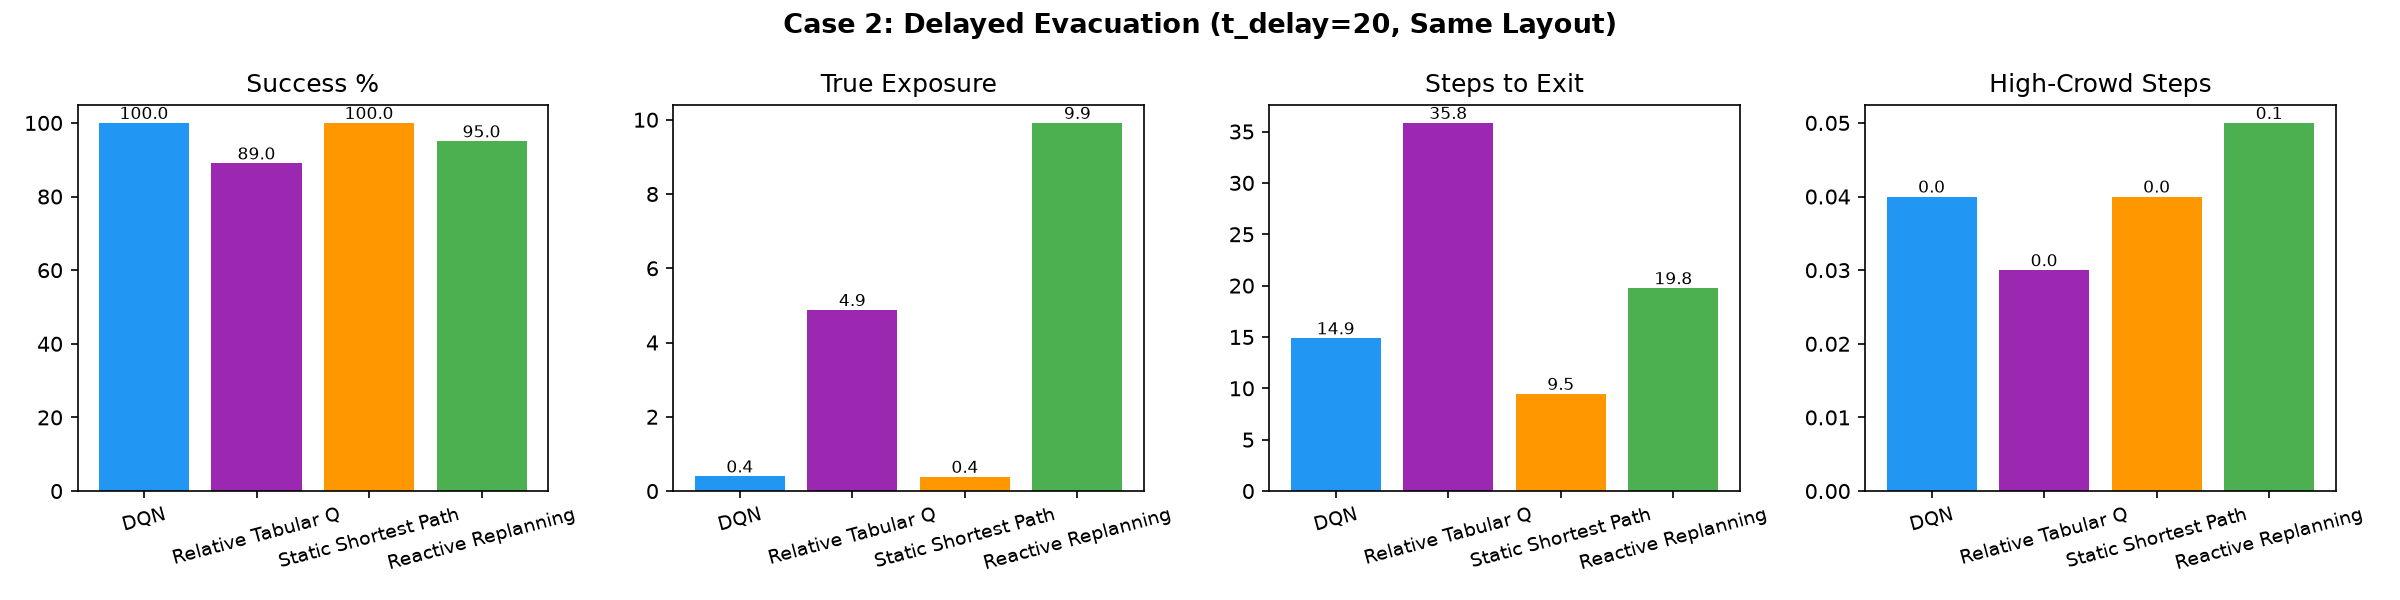
\includegraphics[width=\columnwidth,height=1.05in]{case2_comparison.png}
  \vspace{-0.6em}
  \caption{\textbf{Case 2 Benchmark ($t_{\mathrm{delay}} = 20$ steps on \texttt{layouts/case1.txt}, 100 eps).} DQN achieves 100\% success and 0.06 post-delay exposure, outperforming Reactive Replanning which oscillates in smoke (95\% success, 9.69 exposure).}
  \label{fig:case2}
  \vspace{-0.6em}
\end{figure}

\begin{table}[t]
\centering\scriptsize
\setlength{\tabcolsep}{2.5pt}
\renewcommand{\arraystretch}{0.88}
\caption{Benchmark results across Cases 1, 2, and 3 (100 episodes per method, 5 seeds). Post-delay exposure ($E_{\mathrm{post}}$) isolates active egress performance from stationary delay contamination.}
\label{tab:results}
\begin{tabular}{lcccc}
\toprule
\textbf{Method} & \textbf{Succ.\%} & \textbf{Post Exp} & \textbf{Tot Exp} & \textbf{Steps} \\
\midrule
\multicolumn{5}{l}{\textit{Case 1: Immediate Evacuation ($t_{\mathrm{delay}}=0$, \texttt{layouts/case1.txt})}} \\
DQN (Ours)           & \textbf{100.0} & \textbf{0.08} & \textbf{0.08} & 17.4 \\
Relative Tabular Q   & 100.0          & 0.33          & 0.33          & 23.9 \\
Static Shortest Path & 100.0          & 0.13          & 0.13          & 9.4  \\
Reactive Replanning  & 100.0          & 0.12          & 0.12          & 10.1 \\
\midrule
\multicolumn{5}{l}{\textit{Case 2: Delayed Evacuation ($t_{\mathrm{delay}}=20$, \texttt{layouts/case1.txt})}} \\
DQN (Ours)           & \textbf{100.0} & \textbf{0.06} & \textbf{0.39} & 14.9 \\
Relative Tabular Q   & 89.0           & 4.66          & 4.88          & 35.8 \\
Static Shortest Path & 100.0          & 0.23          & 0.38          & 9.5  \\
Reactive Replanning  & 95.0           & 9.69          & 9.91          & 19.8 \\
\midrule
\multicolumn{5}{l}{\textit{Case 3: Zero-Shot Transfer ($t_{\mathrm{delay}}=0$, \texttt{layouts/case2.txt})}} \\
DQN (Ours)           & 25.0           & 48.42         & 48.42         & 151.9 \\
Relative Tabular Q   & 24.0           & 57.19         & 57.19         & 153.4 \\
Static Shortest Path & 100.0          & 0.03          & 0.03          & 10.7  \\
Reactive Replanning  & 99.0           & 1.83          & 1.83          & 12.9  \\
\bottomrule
\end{tabular}
\vspace{-0.6em}
\end{table}

\subsection{Case 1: Baseline Immediate Evacuation}
Case 1 evaluates immediate egress ($t_{\mathrm{delay}} = 0$) on \texttt{case1.txt} ($9 \times 30$, 2 exits, fire origin $(4, 22)$) under sensor degradation ($\sigma = 0.1, \tau = 2$). As shown in Table~\ref{tab:results}, all four methods achieve 100\% success. Graph baselines exploit global BFS to finish in 9.4--10.1 steps. However, DQN discovers an active risk-averse policy, navigating around hazardous corridor fringes to achieve lower exposure ($0.08$) than Static SP ($0.13$).

\subsection{Case 2: Delayed Evacuation with Corridor Engulfment}
Case 2 imposes a 20-step pre-evacuation delay, during which fire expands from $r=0.95\,\mathrm{m}$ to $2.38\,\mathrm{m}$, engulfing the hallway. DQN demonstrates superior resilience (Table~\ref{tab:results}, Fig.~\ref{fig:case2}): 100\% success and 0.06 post-delay exposure (total 0.39). Reactive Replanning wavers due to belief staleness (95.0\% success, 9.69 post-delay exposure), while Relative Tabular Q drops to 89.0\% success.

\subsection{Case 3: Zero-Shot Cross-Layout Transfer}
Case 3 evaluates policies trained on Case 1 zero-shot on an unseen layout (\texttt{case2.txt}, $13 \times 36$, 4 exits, multi-wing corridors) with zero retraining.

DQN achieves 25.0\% and Relative Tabular Q achieves 24.0\% success (Table~\ref{tab:results}). Both learned methods transfer local navigation skills (following exit bearings, avoiding immediate walls), but fail when non-convex dead ends require backtracking beyond sensing radius $\rho{=}2$. In contrast, Static SP (100\%) and Reactive Replanning (99\%) succeed by computing global paths over the known topology, highlighting the boundary between local perception-action RL and global graph search.

\subsection{Sensor Degradation Sensitivity Sweep}
Sweeping noise ($\sigma \in [0.0, 0.3]$) and latency ($\tau \in [0, 10]$) on Case 1 demonstrates RL robustness. At $\sigma = 0.3$, Static SP degrades to 87.5\% success with 3.74 exposure (Reactive: 4.21 exposure), whereas DQN sustains 97.9\% success with 2.59 exposure. Under crowd panic and herding ($p_{\mathrm{panic}} = p_{\mathrm{herd}} = 0.3$), DQN maintains 0.09 exposure (vs.\ 0.70 for tabular Q), confirming the efficacy of its continuous congestion features.

\section{Limitations and Physical Disclaimer}
\textbf{Hazard Model:} The sigmoidal radial model is an analytical tenability proxy ($O(1)$ query complexity), not a numerical CFD/FDS fire simulation or validated Fractional Effective Dose (FED) model.

\textbf{Delay Parameterization:} The 20-step delay is a chosen simulation parameter designed to induce corridor bottlenecks. Time conversion ($1\text{ step} \approx 1\text{ s}$) is an unvalidated nominal assumption based on $1.0\,\mathrm{m}$ cells and $1.0\,\mathrm{m/s}$ walking speed.

\section{Conclusion}
SafeExit-RL demonstrates that deep reinforcement learning with continuous relative state representations achieves robust, risk-averse fire evacuation guidance under degraded sensing and dynamic corridor bottlenecks where classical heuristics fail. Future work will combine local RL perception with global topological memory.

\clearpage

\begin{thebibliography}{9}
\bibitem{safestep}
H.~Fang, P.~Lin, and S.~Gao, ``Development of a tenability-based path planning model for building fire evacuations using reinforcement learning,'' \emph{Journal of Building Engineering}, vol.~118, p.~115132, 2026.

\bibitem{dqn}
V.~Mnih, K.~Kavukcuoglu, D.~Silver, A.~A. Rusu, et al., ``Human-level control through deep reinforcement learning,'' \emph{Nature}, vol.~518, no.~7540, pp.~529--533, 2015.

\bibitem{rl_evacuation}
C.~Chu, J.~Chen, and Q.~Xu, ``Reinforcement learning based pedestrian evacuation with social force model,'' in \emph{Proc. IEEE ICRA}, 2019, pp.~7532--7538.

\bibitem{pomdp_planning}
D.~Silver and J.~Veness, ``Monte-Carlo planning in large POMDPs,'' in \emph{NeurIPS}, vol.~23, 2010, pp.~2164--2172.

\bibitem{marl_evacuation}
Z.~Shi, E.~Zlatanova, and A.~Kievits, ``Multi-agent reinforcement learning for building evacuation under dynamic fire hazards,'' \emph{Automation in Construction}, vol.~132, p.~103930, 2021.

\bibitem{social_force}
D.~Helbing and P.~Molnar, ``Social force model for pedestrian dynamics,'' \emph{Physical Review E}, vol.~51, no.~5, pp.~4282--4286, 1995.
\end{thebibliography}

\end{document}
